\clearpage
\subsection{ШИМ}
ШИМ на  рис.\ref{fig:sim_final_VSS_PWM}. 
\begin{figure}[!h]\centering
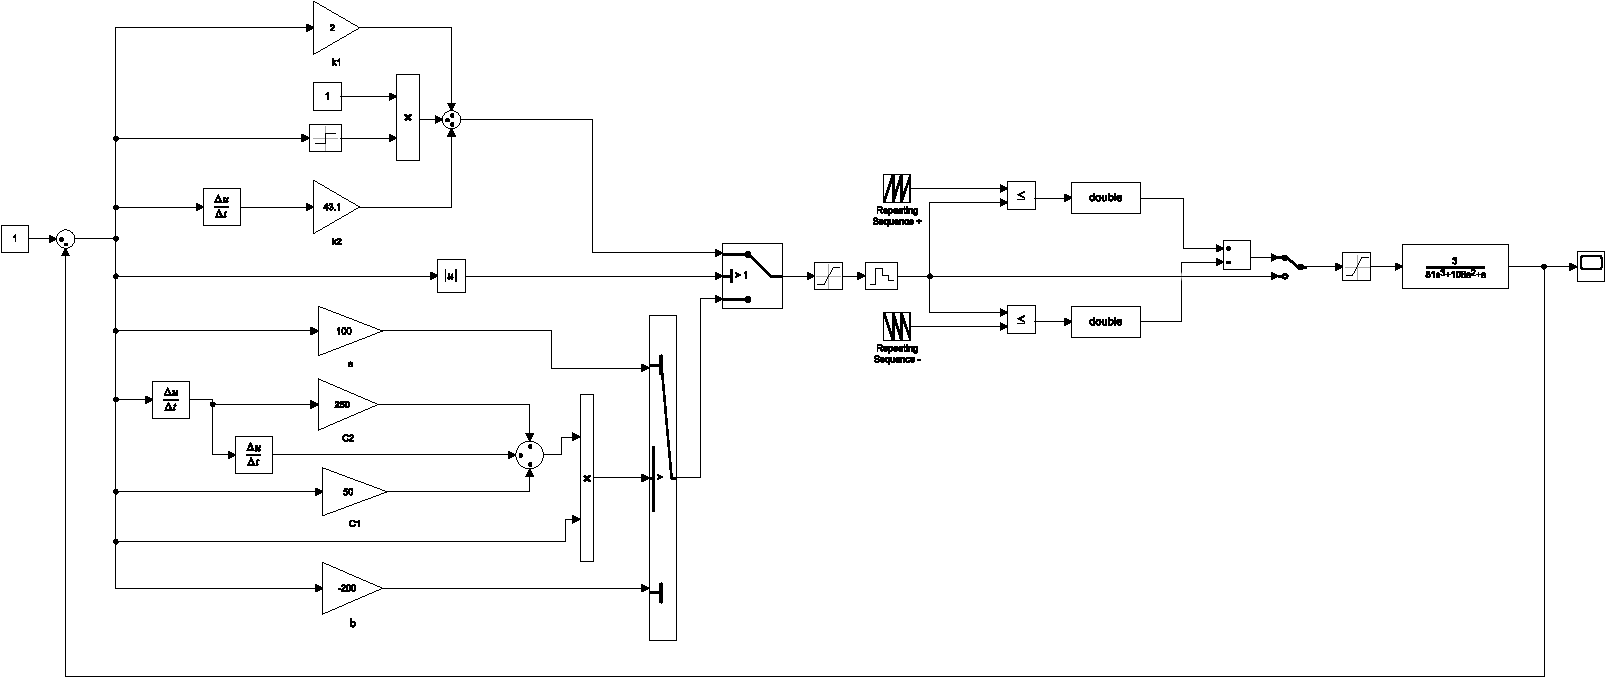
\includegraphics[width=1.0\linewidth]{images/sim_final_VSS_PWM}
\caption{Структурная схема нелинейной СПС с ШИМ. }\label{fig:sim_final_VSS_PWM}
\end{figure}

в результате видим, что переходный процесс не изменился
\begin{figure}[!h]\centering
\includegraphics[width=0.6\linewidth]{images/final_VSS_PWM_DCS_SAWnew}
\caption{ Переворачиваем пилу  и поднимаем её над осью абсцис}\label{fig:final_VSS_PWM_DCS_SAWnew}
\end{figure}
\begin{figure}[!h]\centering
\includegraphics[width=0.6\linewidth]{images/final_VSS_PWM_DCS_pwm1}
\caption{ ШИМ1}\label{fig:final_VSS_PWM_DCS_pwm1}
\end{figure}
\begin{figure}[!h]\centering
\includegraphics[width=0.6\linewidth]{images/final_VSS_PWM_DCS_pwm2}
\caption{ ШИМ2}\label{fig:final_VSS_PWM_DCS_pwm2}
\end{figure}
\begin{figure}[!h]\centering
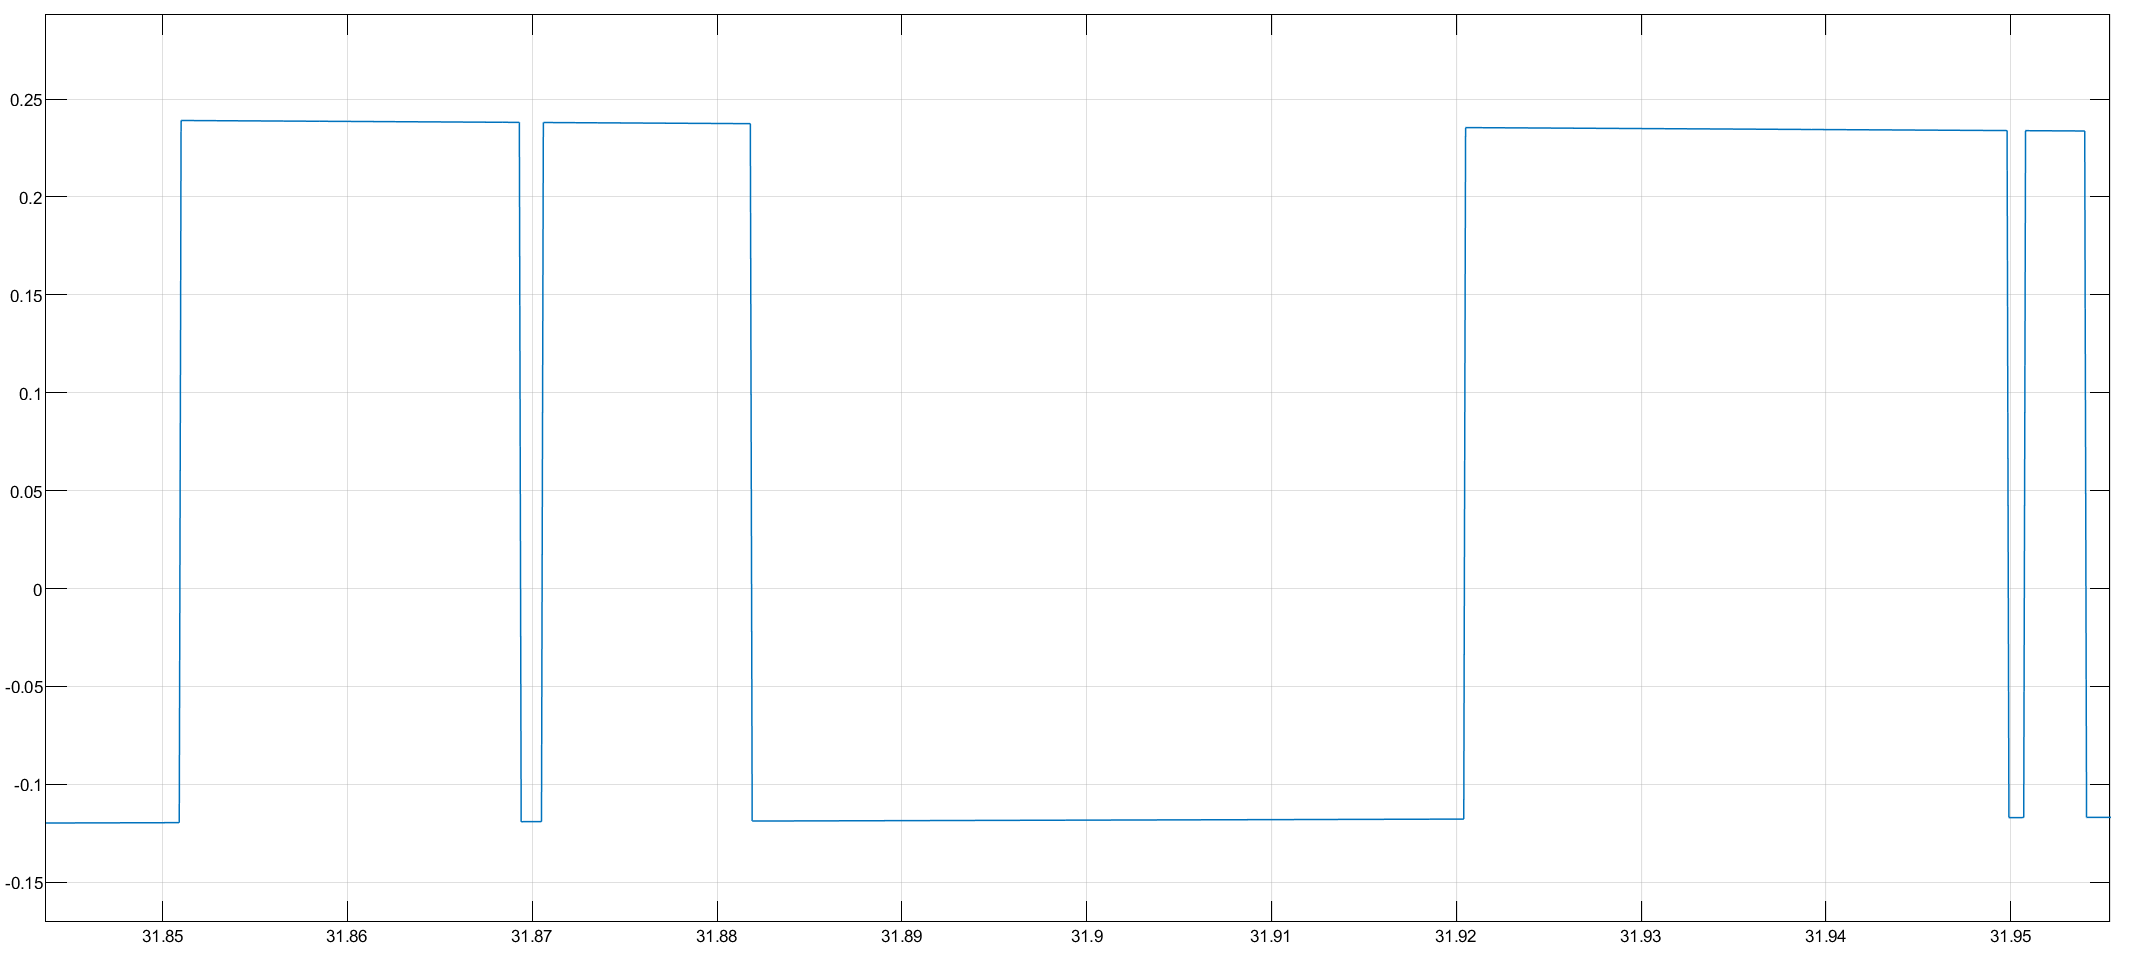
\includegraphics[width=0.6\linewidth]{images/final_VSS_PWM_DCS_upr}
\caption{ управляющий непрерывный сигнал }\label{fig:final_VSS_PWM_DCS_upr}
\end{figure}
\begin{figure}[!h]\centering
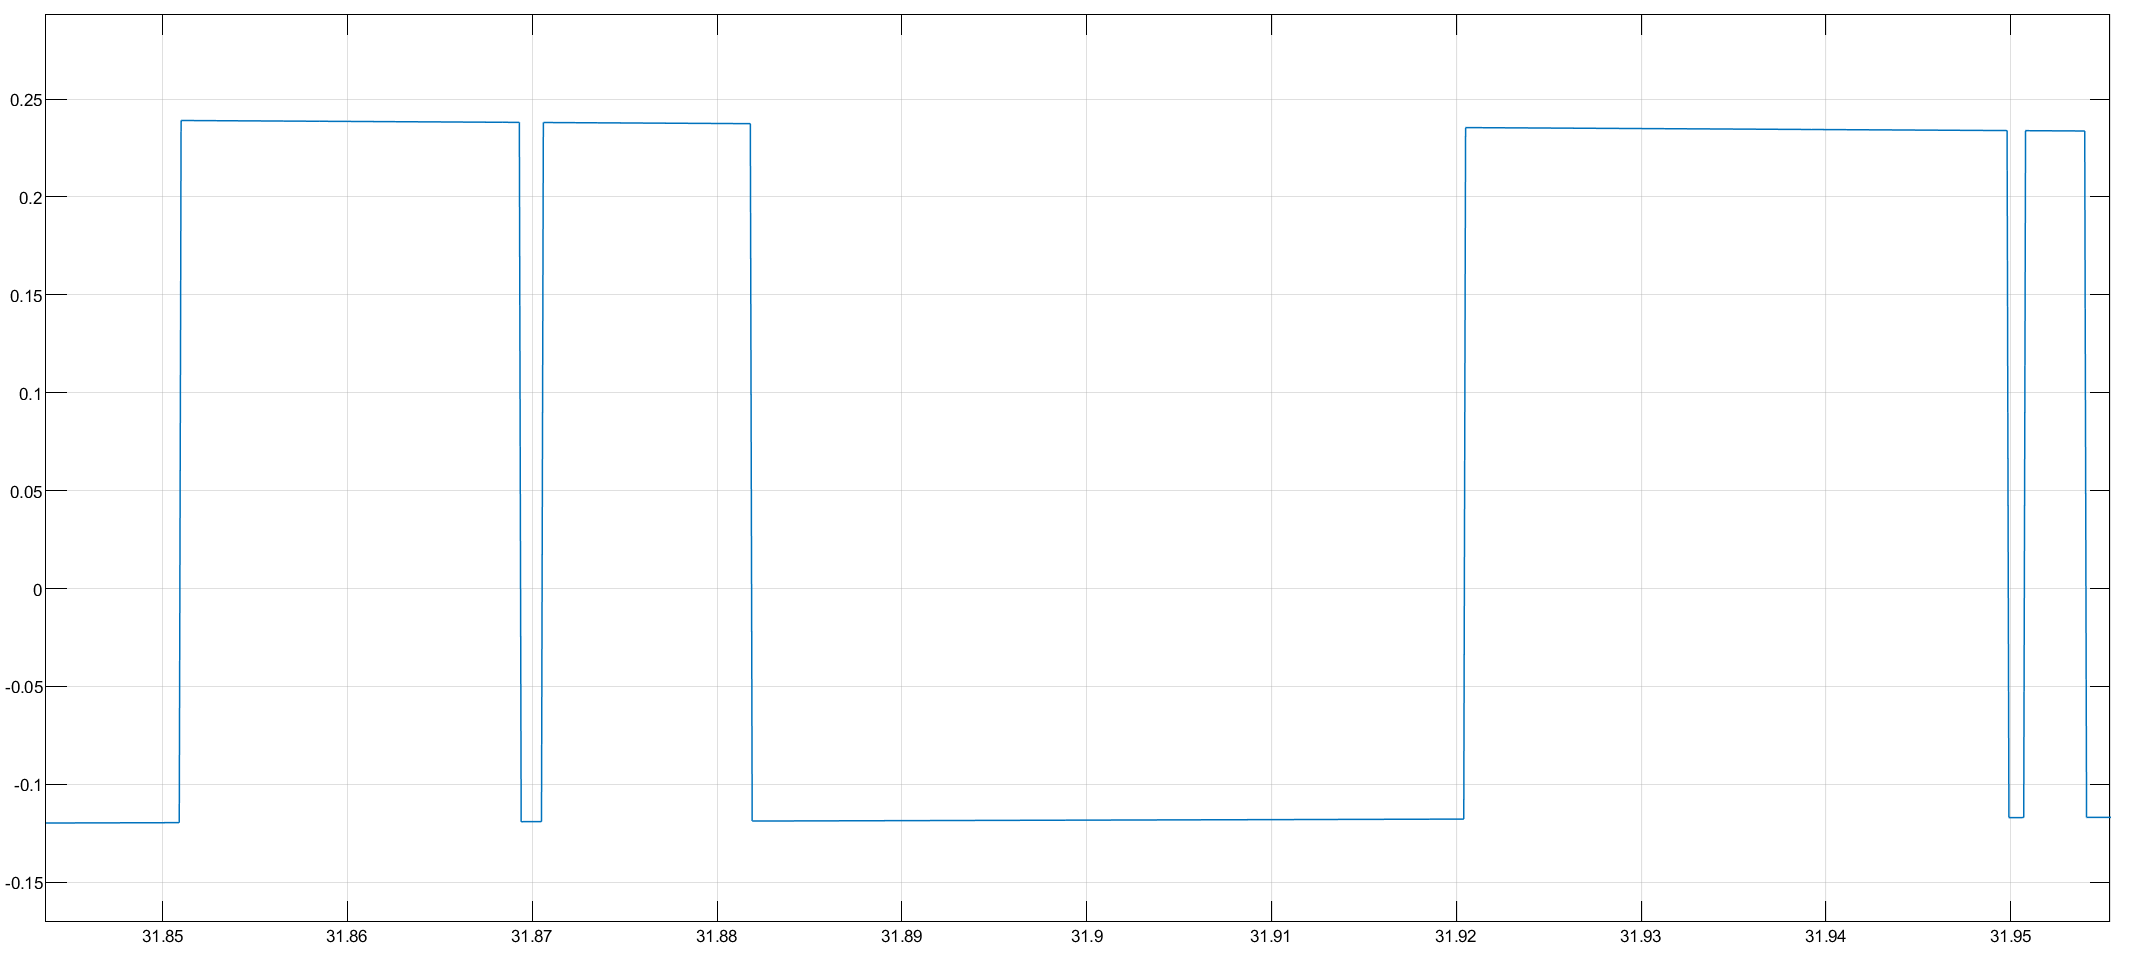
\includegraphics[width=0.6\linewidth]{images/final_VSS_PWM_DCS_upr_ogr}
\caption{ управляющий непрерывный сигнал после насыщения}\label{fig:final_VSS_PWM_DCS_upr_ogr}
\end{figure}

